Both cytoplasmic and periplasmic proteins seem to have a maximum in distribution around the length of 220,
and both distribution display an positive skewness toward larger proteins lengths (Fig. \ref{fig:protein_lengths_graph})
The cytoplasmic distribution is more evenly spread around a wider range of protein lengths.
The periplasmic distribution on the other hand displays sharper peaks.
On average, 
periplasmic proteins are shorter than cytoplasmic ones,
as was determined with a Wilcoxon-ranksum test (p-value 2e-24).
This difference in length was also observed by \cite{loos2019} in \textit{Escherichia coli},
but seems to hold true for Gammaproteobacteria in general.
The maximum length observed in cytoplasmic proteins was 3326,
for periplasmic proteins this was only 1849 (Fig. \ref{fig:protein_lengths_table}).
Additionally, the histogram shows that protein with a length higher than 600 occur more frequently in the cytoplasm than periplasm.

~\begin{figure}[h!]
	~\begin{subfigure}[b]{0.3\linewidth}
		~\begin{longtable}[]{@{}lll@{}}
			\toprule
			& Cytoplasm & Periplasm\tabularnewline
			\midrule
			\endhead
			count & 30632 & 3883\tabularnewline
			mean & 336 & 286\tabularnewline
			std & 212 & 125\tabularnewline
			min & 42 & 78\tabularnewline
			25\% & 200 & 213\tabularnewline
			50\% & 283 & 244\tabularnewline
			75\% & 409 & 330\tabularnewline
			max & 3326 & 1849\tabularnewline
			\bottomrule
		~\end{longtable}
		\caption{}
		\label{fig:protein_lengths_table}
	~\end{subfigure}
	\hfill
	~\begin{subfigure}[b]{0.68\linewidth}
		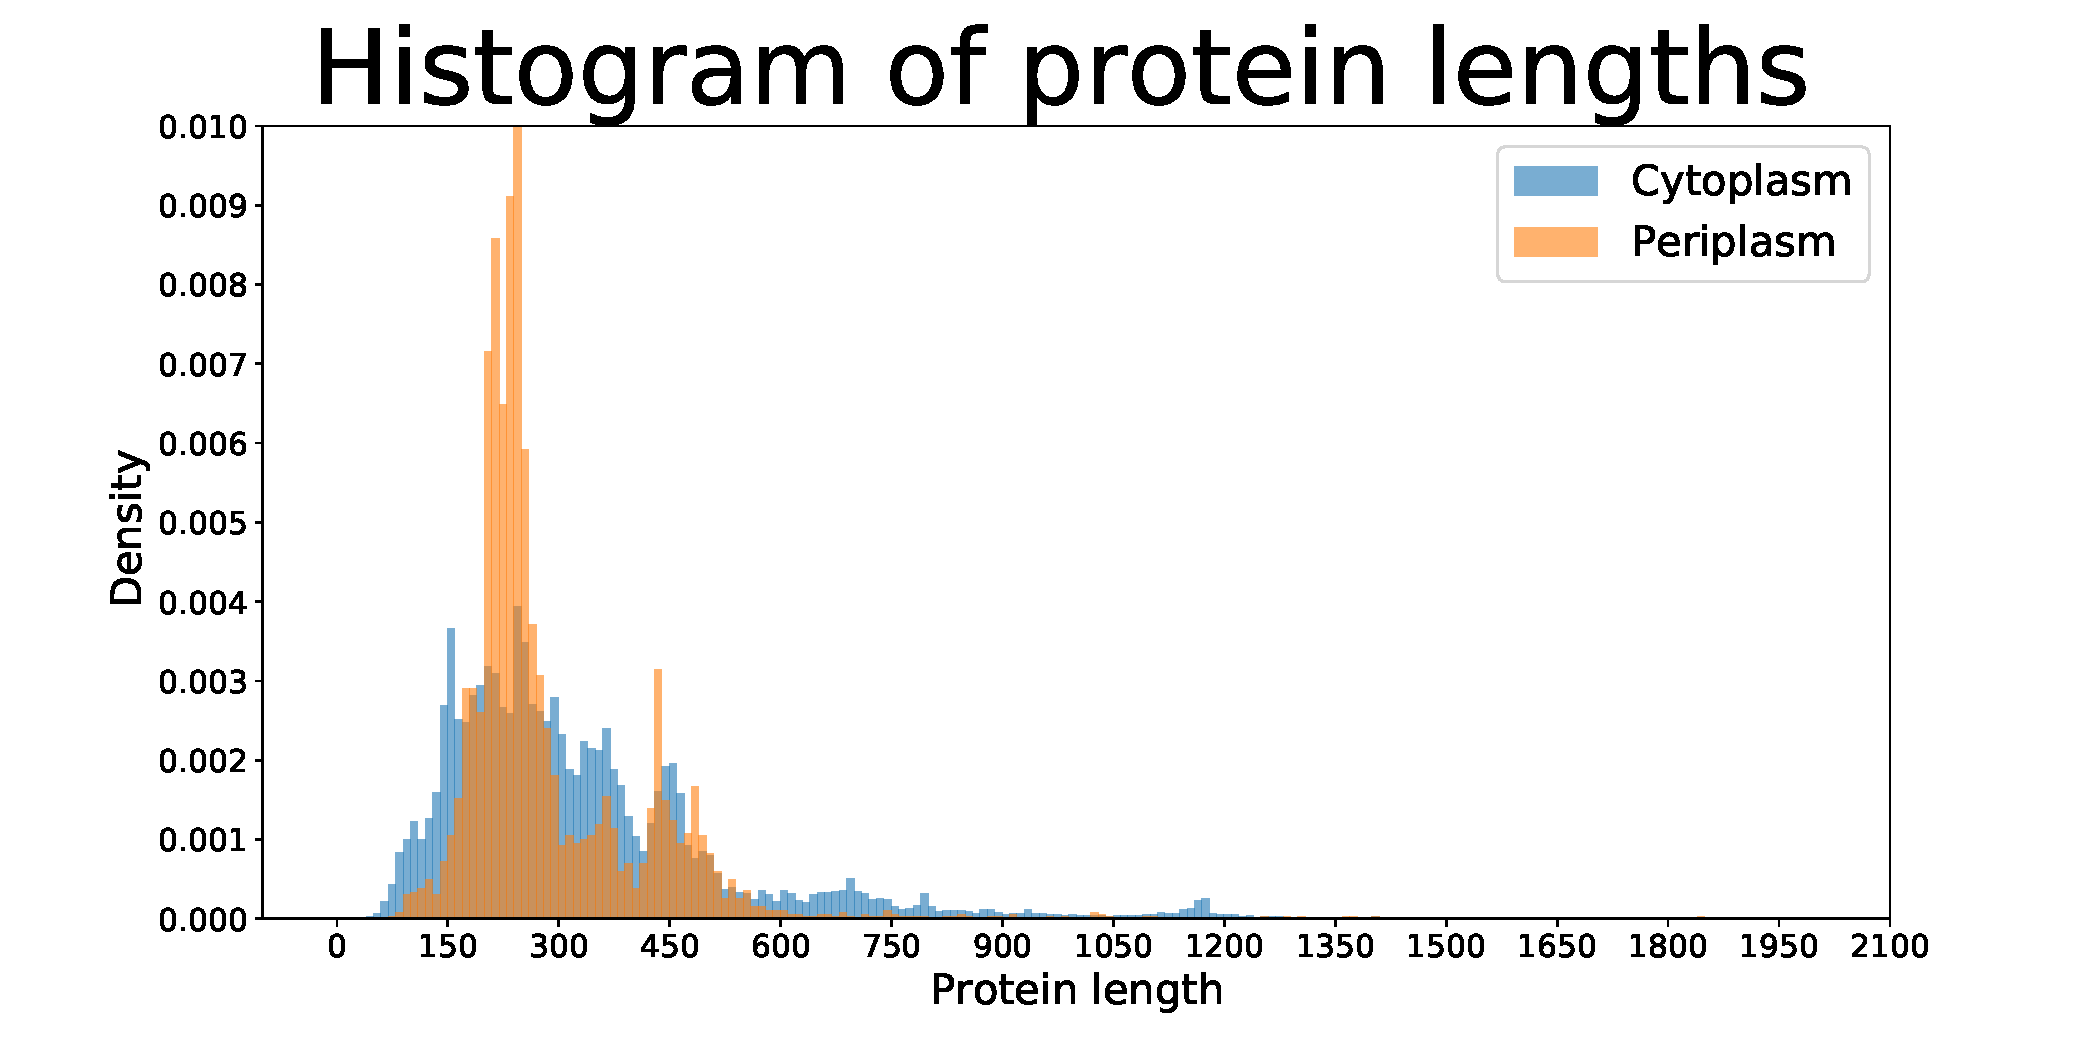
\includegraphics[width=\linewidth]
{./results/general_comparison/global_comparison/length/img/protein_lengths.pdf}
		\caption{}
		\label{fig:protein_lengths_graph}
	~\end{subfigure}
	\caption{
	\textbf{Comparison of protein length distributions between cytoplasmic and periplasmic proteins.}
	}
	\label{fig:protein_lengths}
~\end{figure}
